% Options for packages loaded elsewhere
\PassOptionsToPackage{unicode}{hyperref}
\PassOptionsToPackage{hyphens}{url}
\PassOptionsToPackage{dvipsnames,svgnames*,x11names*}{xcolor}
%
\documentclass[
  10pt,
]{article}
\usepackage{lmodern}
\usepackage{setspace}
\usepackage{amssymb,amsmath}
\usepackage{ifxetex,ifluatex}
\ifnum 0\ifxetex 1\fi\ifluatex 1\fi=0 % if pdftex
  \usepackage[T1]{fontenc}
  \usepackage[utf8]{inputenc}
  \usepackage{textcomp} % provide euro and other symbols
\else % if luatex or xetex
  \usepackage{unicode-math}
  \defaultfontfeatures{Scale=MatchLowercase}
  \defaultfontfeatures[\rmfamily]{Ligatures=TeX,Scale=1}
  \setmainfont[]{DejaVu Serif}
  \setmonofont[]{DejaVu Sans Mono}
\fi
% Use upquote if available, for straight quotes in verbatim environments
\IfFileExists{upquote.sty}{\usepackage{upquote}}{}
\IfFileExists{microtype.sty}{% use microtype if available
  \usepackage[]{microtype}
  \UseMicrotypeSet[protrusion]{basicmath} % disable protrusion for tt fonts
}{}
\makeatletter
\@ifundefined{KOMAClassName}{% if non-KOMA class
  \IfFileExists{parskip.sty}{%
    \usepackage{parskip}
  }{% else
    \setlength{\parindent}{0pt}
    \setlength{\parskip}{6pt plus 2pt minus 1pt}}
}{% if KOMA class
  \KOMAoptions{parskip=half}}
\makeatother
\usepackage{xcolor}
\IfFileExists{xurl.sty}{\usepackage{xurl}}{} % add URL line breaks if available
\IfFileExists{bookmark.sty}{\usepackage{bookmark}}{\usepackage{hyperref}}
\hypersetup{
  colorlinks=true,
  linkcolor=red,
  filecolor=red,
  citecolor=red,
  urlcolor=red,
  pdfcreator={LaTeX via pandoc}}
\urlstyle{same} % disable monospaced font for URLs
\usepackage[margin=0.7cm,top=0.7cm,bottom=0.7cm,left=0.7cm,right=0.7cm,includeheadfoot]{geometry}
\usepackage{graphicx}
\makeatletter
\def\maxwidth{\ifdim\Gin@nat@width>\linewidth\linewidth\else\Gin@nat@width\fi}
\def\maxheight{\ifdim\Gin@nat@height>\textheight\textheight\else\Gin@nat@height\fi}
\makeatother
% Scale images if necessary, so that they will not overflow the page
% margins by default, and it is still possible to overwrite the defaults
% using explicit options in \includegraphics[width, height, ...]{}
\setkeys{Gin}{width=\maxwidth,height=\maxheight,keepaspectratio}
% Set default figure placement to htbp
\makeatletter
\def\fps@figure{htbp}
\makeatother
\setlength{\emergencystretch}{3em} % prevent overfull lines
\providecommand{\tightlist}{%
  \setlength{\itemsep}{0pt}\setlength{\parskip}{0pt}}
\setcounter{secnumdepth}{3}
% Enable graphics inclusion and ensure figure numbering works
\usepackage{graphicx}
\renewcommand{\figurename}{Figure}

% Configure fonts for Unicode support with fallbacks
\usepackage{newunicodechar}
\newunicodechar{⁴}{\textsuperscript{4}}
\newunicodechar{₄}{\textsubscript{4}}

% Configure hyperref colors consistently
\AtBeginDocument{
% Override pandoc's hidelinks setting with consistent options
\hypersetup{
    colorlinks=true,
    allcolors=red,
    linkcolor=red,
    urlcolor=red,
    citecolor=red,
    filecolor=red,
    menucolor=red,
    linktoc=all
}
}

\title{Introduction}
\author{Daniel Ari Friedman\\ ORCID: 0000-0001-6232-9096\\ Email: daniel@activeinference.institute}
\date{August 14, 2025}

\begin{document}
\maketitle

{
\hypersetup{linkcolor=red}
\setcounter{tocdepth}{3}
\tableofcontents
}
\setstretch{1.0}
\hypertarget{introduction}{%
\section{Introduction}\label{introduction}}

Quadray coordinates provide a tetrahedral basis for modeling space and
computation, standing in contrast to Cartesian frameworks. Originating
in Buckminster Fuller's Synergetics, quadray coordinates enable the
replacement of right-angle assumptions, with 60-degree coordination and
a unit tetrahedron of volume 1. This reframing yields striking integer
relationships among common polyhedra and provides a natural account of
space via close-packed spheres and the isotropic vector matrix (IVM).

In this synthetic review, we distinguish three internal meanings of
``4D,'' following a dot-notation that avoids cross-domain confusion:

\begin{itemize}
\tightlist
\item
  Coxeter.4D --- four-dimensional Euclidean space (E⁴), as in classical
  polytope theory. Coxeter emphasizes that Euclidean 4D is not
  spacetime; see the Dover edition of Regular Polytopes (p.~119) for a
  clear statement to this effect; background on lattice packings in four
  dimensions aligns with the treatment in Conway \& Sloane's
  \href{https://link.springer.com/book/10.1007/978-1-4757-6568-7}{Sphere
  Packings, Lattices and Groups (Springer)}.
\item
  Einstein.4D --- Minkowski spacetime (3D + time) with an indefinite
  metric; appropriate for relativistic physics but distinct from
  Euclidean E⁴.
\item
  Fuller.4D --- synergetics' tetrahedral accounting of space using
  Quadrays (four non-negative coordinates with at least one zero after
  normalization) and the IVM = CCP = FCC correspondence. This treats the
  regular tetrahedron as a natural unit container and emphasizes
  angle/shape relations independent of time/energy.
\end{itemize}

Kirby Urner's expositions and implementations have been influential in
making Quadray coordinates practical and accessible across multiple
programming languages and educational contexts. See the comprehensive
\href{https://github.com/4dsolutions}{4dsolutions ecosystem}:

\begin{itemize}
\tightlist
\item
  \textbf{Foundational materials}:
  \href{https://www.grunch.net/synergetics/quadintro.html}{Urner --
  Quadray intro},
  \href{https://www.grunch.net/synergetics/quadxyz.html}{Quadrays and
  XYZ}, \href{https://www.grunch.net/synergetics/quadphil.html}{Quadrays
  and the Philosophy of Mathematics}
\item
  \textbf{Python implementations}: Core modules
  \href{https://github.com/4dsolutions/m4w/blob/main/qrays.py}{\texttt{qrays.py}}
  (Quadray vectors with SymPy support) and
  \href{https://github.com/4dsolutions/m4w/blob/main/tetravolume.py}{\texttt{tetravolume.py}}
  (IVM volumes, BEAST modules)
\item
  \textbf{Educational notebooks}:
  \href{https://github.com/4dsolutions/School_of_Tomorrow}{School\_of\_Tomorrow}
  including
  \href{https://github.com/4dsolutions/School_of_Tomorrow/blob/master/Qvolume.ipynb}{Qvolume.ipynb}
  (Tom Ace 5×5) and
  \href{https://github.com/4dsolutions/School_of_Tomorrow/blob/master/VolumeTalk.ipynb}{VolumeTalk.ipynb}
  (bridging vs native)
\item
  \textbf{Cross-language validation}:
  \href{https://github.com/4dsolutions/rusty_rays}{Rust implementation},
  \href{https://github.com/4dsolutions/synmods}{Clojure functional
  approach}, \href{https://github.com/4dsolutions/BookCovers}{VPython
  visualizations}
\item
  \textbf{Historical context}:
  \href{https://mail.python.org/pipermail/edu-sig/2000-May/000498.html}{Python
  edu-sig post (May 2000)}
\end{itemize}

This paper unifies three threads:

\begin{itemize}
\tightlist
\item
  \textbf{Foundations}: Quadray coordinates and their relation to 4D
  modeling more generally, with explicit namespace usage (Coxeter.4D,
  Einstein.4D, Fuller.4D) to maintain clarity.
\item
  \textbf{Optimization framework}: leverages integer volume quantization
  on tetrahedral lattices to achieve robust, discrete convergence.
\item
  \textbf{Information geometry}: tools (e.g., Fisher Information,
  free-energy minimization) for interpreting optimization as geodesic
  motion on statistical manifolds.
\end{itemize}

Contributions:

\begin{itemize}
\tightlist
\item
  \textbf{Namespaces mapping}: Coxeter.4D (Euclidean E⁴), Einstein.4D
  (Minkowski spacetime), and Fuller.4D (Quadrays/IVM) → analytical tools
  and examples.
\item
  \textbf{Quadray-adapted Nelder--Mead}: integer-lattice normalization
  and volume-level tracking.
\item
  \textbf{Equations and methods}: comprehensive supplement with guidance
  for high-precision computation using \texttt{libquadmath}.
\item
  \textbf{Discrete optimizer}: integer-valued variational descent over
  the IVM (\texttt{discrete\_ivm\_descent}) with animation tooling,
  connecting lattice geometry to information-theoretic objectives.
\end{itemize}

\hypertarget{related-work-and-background}{%
\subsection{Related work and
background}\label{related-work-and-background}}

\begin{itemize}
\tightlist
\item
  \textbf{Tetrahedron volume formulas}: length-based
  \href{https://en.wikipedia.org/wiki/Cayley\%E2\%80\%93Menger_determinant}{Cayley--Menger
  determinant} and determinant-based expressions on vertex coordinates
  (see
  \href{https://en.wikipedia.org/wiki/Tetrahedron\#Volume}{Tetrahedron
  -- volume}).
\item
  \textbf{Exact determinants}:
  \href{https://en.wikipedia.org/wiki/Bareiss_algorithm}{Bareiss
  algorithm}, used in our integer tetravolume implementations.
\item
  \textbf{Information geometry}:
  \href{https://en.wikipedia.org/wiki/Fisher_information}{Fisher
  information} and
  \href{https://en.wikipedia.org/wiki/Natural_gradient}{natural
  gradient}.
\item
  \textbf{Optimization baseline}: the
  \href{https://en.wikipedia.org/wiki/Nelder\%E2\%80\%93Mead_method}{Nelder--Mead
  method}, adapted here to the Quadray lattice.
\item
  \textbf{4dsolutions ecosystem (comprehensive implementation suite)}:
  The \href{https://github.com/4dsolutions}{4dsolutions organization}
  provides extensive computational resources for Quadrays and synergetic
  geometry:

  \begin{itemize}
  \tightlist
  \item
    \textbf{Primary Python modules}:
    \href{https://github.com/4dsolutions/m4w/blob/main/qrays.py}{\texttt{qrays.py}}
    (Quadray vector operations, normalization, XYZ bridging) and
    \href{https://github.com/4dsolutions/m4w/blob/main/tetravolume.py}{\texttt{tetravolume.py}}
    (IVM volumes, BEAST modules, multiple algorithms)
  \item
    \textbf{Educational framework}:
    \href{https://github.com/4dsolutions/School_of_Tomorrow}{School\_of\_Tomorrow}
    with interactive tutorials and algorithm comparisons in
    \href{https://github.com/4dsolutions/School_of_Tomorrow/blob/master/Qvolume.ipynb}{Qvolume.ipynb}
    and
    \href{https://github.com/4dsolutions/School_of_Tomorrow/blob/master/VolumeTalk.ipynb}{VolumeTalk.ipynb}
  \item
    \textbf{Cross-platform validation}: Independent implementations in
    \href{https://github.com/4dsolutions/rusty_rays}{Rust},
    \href{https://github.com/4dsolutions/synmods}{Clojure}, POV-Ray
    pipelines
    (\href{https://github.com/4dsolutions/School_of_Tomorrow/blob/master/quadcraft.py}{quadcraft.py}),
    and \href{https://github.com/4dsolutions/BookCovers}{VPython
    animations}
  \end{itemize}
\item
  \textbf{Related work}:
  \href{https://github.com/docxology/quadcraft/}{QuadCraft} is a
  tetrahedral voxel engine game using Quadray coordinates.
\end{itemize}

Ecosystem context: The 4dsolutions organization spans 29+ repositories
with implementations across Python, Rust, Clojure, POV-Ray, and VPython,
providing extensive cross-language validation and educational resources.
Core algorithmic modules include vector operations, volume calculations,
visualization pipelines, and pedagogical frameworks that complement and
validate the methods developed in this manuscript. See the comprehensive
catalog in \texttt{07\_resources.md}.

\hypertarget{companion-code-and-tests}{%
\subsection{Companion code and tests}\label{companion-code-and-tests}}

The manuscript is accompanied by a fully-tested Python codebase under
\texttt{src/} with unit tests under \texttt{tests/}. Key artifacts used
throughout the paper:

\begin{itemize}
\tightlist
\item
  \textbf{Quadray APIs}: \texttt{src/quadray.py} (\texttt{Quadray},
  \texttt{integer\_tetra\_volume}, \texttt{ace\_tetravolume\_5x5}).
\item
  \textbf{Determinant utilities}: \texttt{src/linalg\_utils.py}
  (\texttt{bareiss\_determinant\_int}).
\item
  \textbf{Length-based volume}: \texttt{src/cayley\_menger.py}
  (\texttt{tetra\_volume\_cayley\_menger},
  \texttt{ivm\_tetra\_volume\_cayley\_menger}).
\item
  \textbf{XYZ conversion}: \texttt{src/conversions.py}
  (\texttt{urner\_embedding}, \texttt{quadray\_to\_xyz}).
\item
  \textbf{Examples}: \texttt{src/examples.py}
  (\texttt{example\_ivm\_neighbors}, \texttt{example\_volume},
  \texttt{example\_optimize}).
\end{itemize}

Figure 1 (graphical abstract): Panel A shows Quadray axes (A,B,C,D)
under a symmetric embedding with wireframe context. Panel B shows
close-packed spheres at the tetrahedron vertices (IVM/CCP/FCC, ``twelve
around one'').

\begin{figure}
\centering
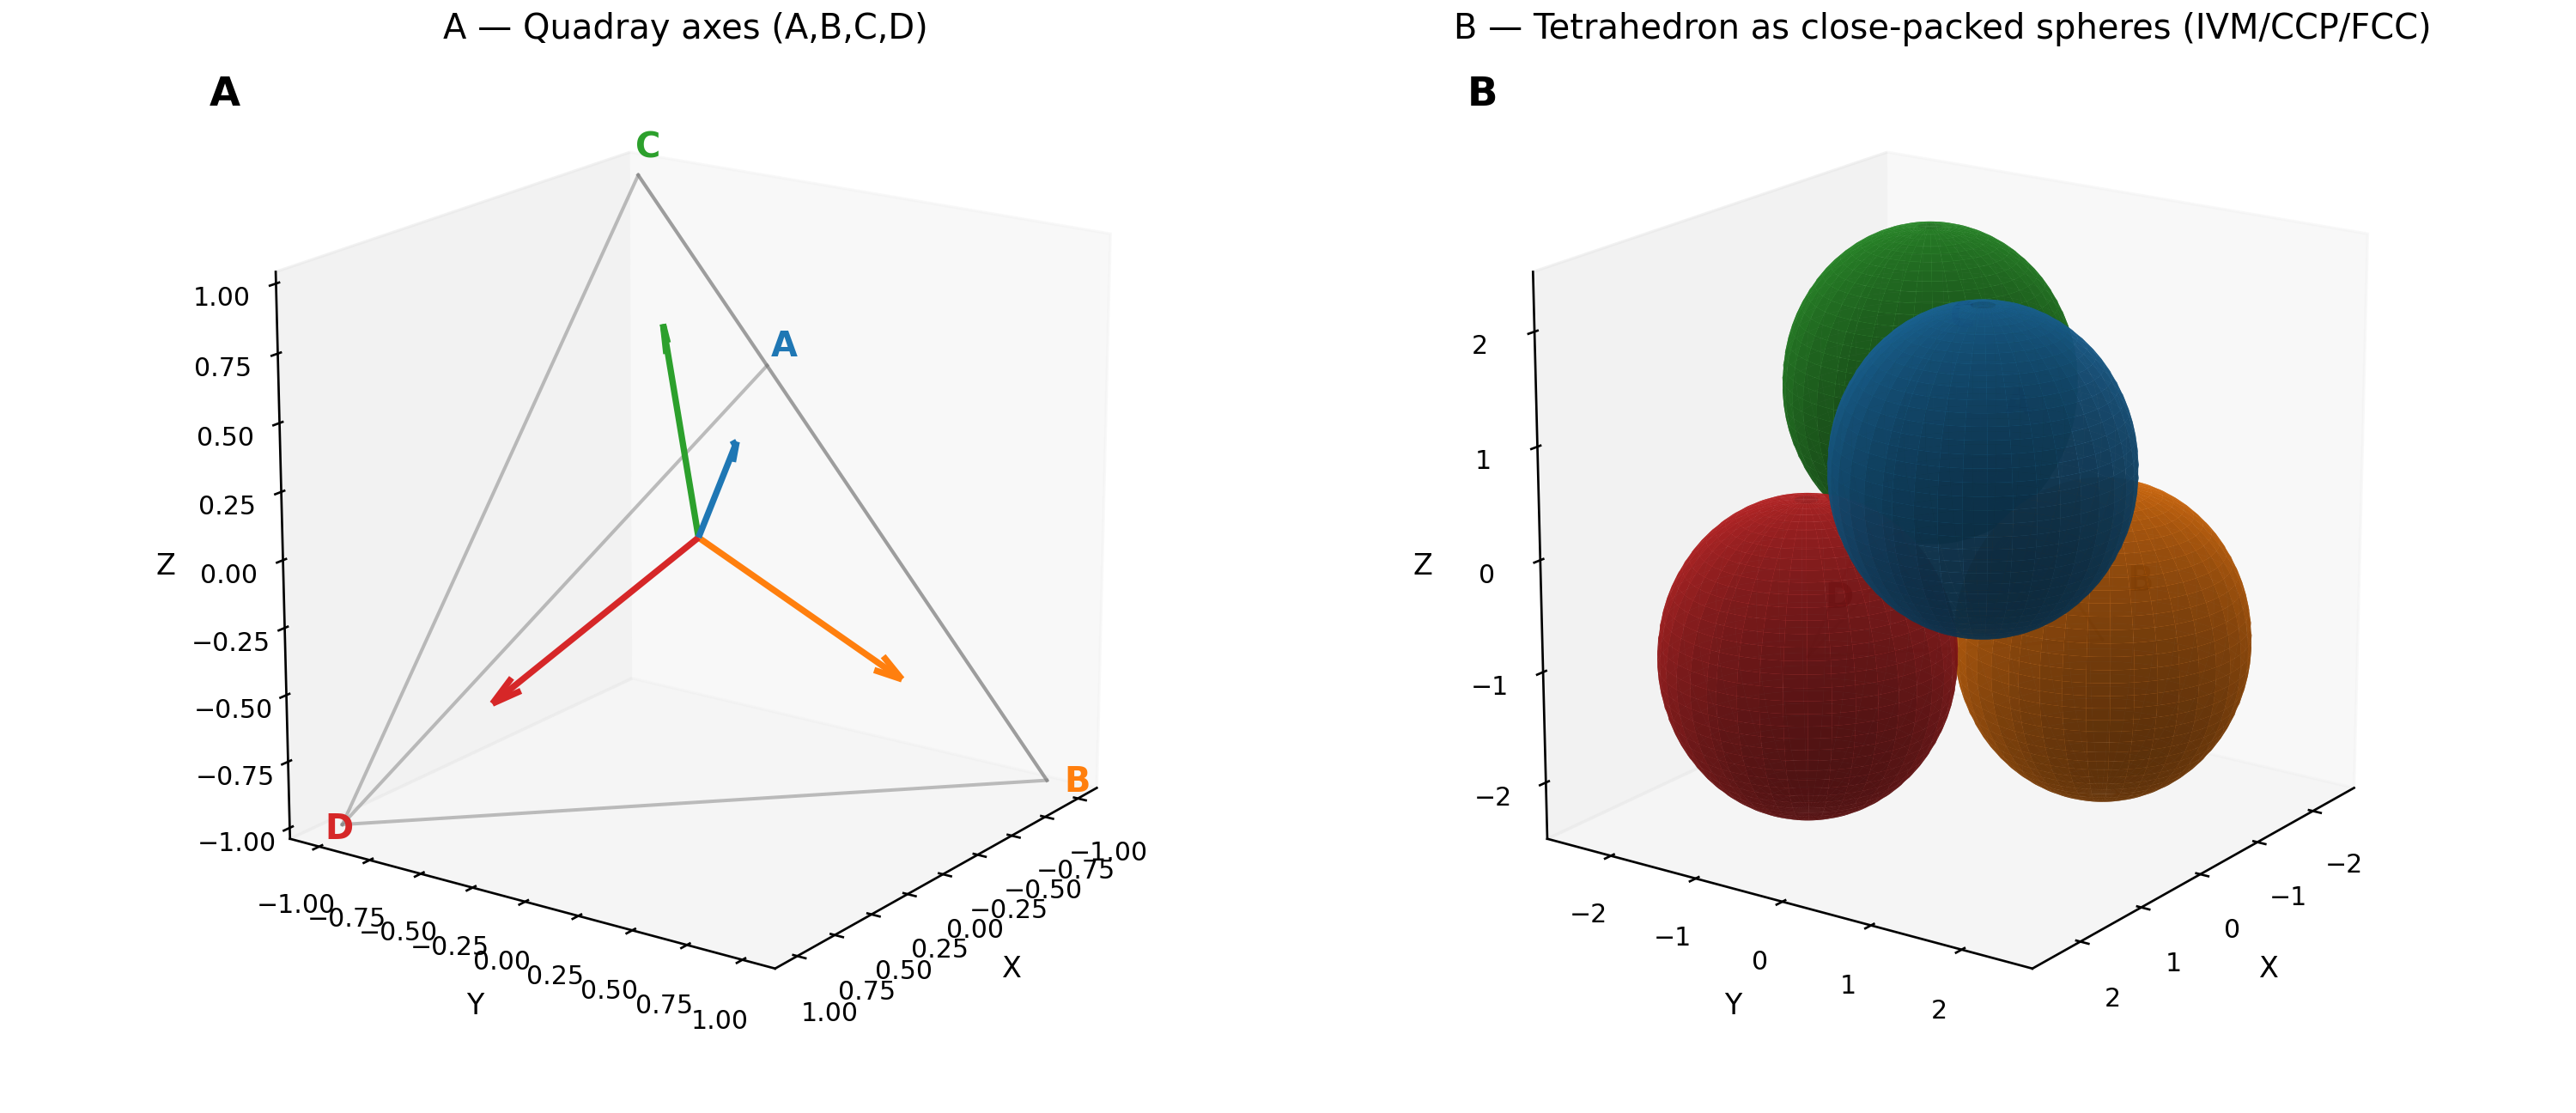
\includegraphics{figures/graphical_abstract_quadray.png}
\caption{\textbf{Figure 1: Quadray coordinate system overview (graphical
abstract)}. \textbf{Panel A}: Four Quadray axes (A,B,C,D) rendered as
colored directional arrows from the origin to the vertices of a regular
tetrahedron under the default symmetric embedding. Each axis is
distinctly colored (A=blue, B=orange, C=green, D=red) with axis labels
positioned at the vertex endpoints. A light gray wireframe connects the
four vertices to emphasize the tetrahedral geometry underlying the
coordinate system. This panel illustrates the fundamental Fuller.4D
direction-based structure where Quadrays represent four canonical
directions in tetrahedral space rather than orthogonal Cartesian
dimensions. \textbf{Panel B}: The same tetrahedral vertices shown as
close-packed spheres with radius chosen so neighboring spheres kiss
along tetrahedron edges, emphasizing the connection to the Isotropic
Vector Matrix (IVM), Cubic Close Packing (CCP), and Face-Centered Cubic
(FCC) arrangements. Each sphere is colored to match its corresponding
axis from Panel A, with light edge wireframes providing geometric
context. This visualization demonstrates how Quadray coordinates
naturally align with dense sphere packing and the ``twelve around one''
coordination motif central to synergetics and Fuller.4D modeling.}
\end{figure}

Tests illustrate expected behavior and edge cases (see \texttt{tests/}),
and coverage is enforced at 100\% for \texttt{src/}.

\end{document}
